\section{Motivation} \label{sec:motivation}
High level synthesis tools greatly alleviaite the efforts of building BFS accelerators on FPGAs. 
Nevertheless, the performance of the resulting accelerators can be far from satisfying 
especially for irregular applications like BFS. In this section, we take our own experience 
on optimizing BFS using HLS on Alpha-Data as an example and show the challenge to 
optimize BFS using HLS tools.

We started from basic sequential BFS algorithm as listed in Algorithm \ref{alg:bfs} for 
the HLS design. First of all, we separated the nested loop into different pipeling 
stages connected via FIFO using data flow model supported by Xilinx HLS. 
We explored all the possible pipelining combinations ranging from single-stage 
pipeline to seven-stage pipeline. With the optimized pipelining, we further 
introduced pre-fetch buffer to improve memory access efficiency, 
added customized cache structure for the vertex property to reduce the external 
memory accesses, hash table based redundancy removal logic to reduce the repeated 
outgoing neighboring vertices of the frontier vertices. Finally, we also tried to 
duplicate the pipeline stages for parallel processing and tuned the design paramters 
of the accelerators such as cache and pre-fetch buffer size. Up to now, we believe 
we have tried the major design optimization methods that can be applied to the 
baseline HLS design. 

\begin{algorithm}
	\caption{BFS Algorithm} \label{alg:bfs}
    \small
	\begin{algorithmic}[1]
		\Procedure{BFS}{}
		\State $level[v_k] \gets -1$ where $v_k \in V$
		\State $level[v_s] \gets 0$
		\State $current\_level \gets 0$
		\State $frontier \gets v_s$

        \While {$!frontier.empty()$} 

		\For{$v \in V$}
		\If{$level[v] == current\_level$}
		\State $frontier \gets v$
		\EndIf
		\EndFor

		\For{$v \in frontier$}
		\State $S \gets {n \in V | (v, n) \in E}$
		\For {$n \in S$}
		\If {$level[n] == -1$}
		\State $level[n] \gets current\_level + 1$
		\EndIf
		\EndFor
		\EndFor
		\State $current\_level \gets current\_level + 1$
		\EndWhile
		\EndProcedure
	\end{algorithmic}
\end{algorithm}

We measured the performance of the accelerator with a set of representative graphs 
including Youtube, Live Journal, Orkut and two R-MAT graphs. Details about the 
graph benchmark can be found in xxx. Figure \ref{fig:opt-performance} presents the performance improvement 
when different optimization techqniues are gradually applied to the baseline design.
It can be found that the resulting BFS accelerator achieves up to 70X performance speedup
compared to the baseline design. It indicates that the HLS optimizations help improve the 
performance significantly. However, when the accelerator is compread to the existing 
handcrafted design reported in prior work, it can be found that it remains 
far from satisfying as shown in Table \ref{tab:compare}.
\begin{figure}
\center{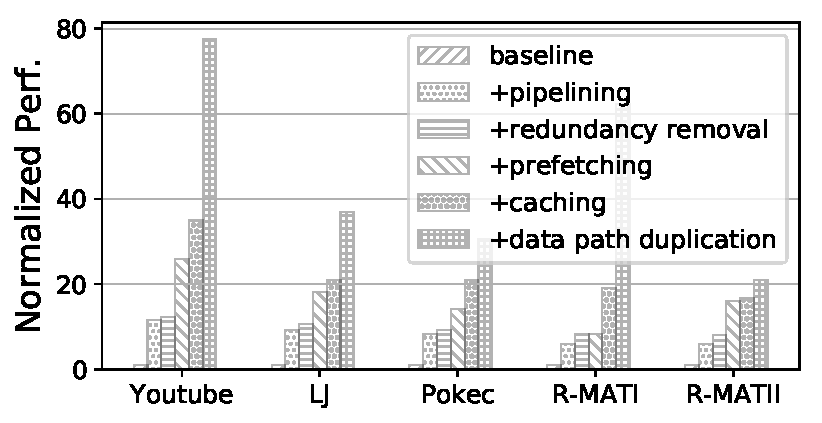
\includegraphics[width=0.95\linewidth]{opt-performance}}
    \caption{BFS accelerator optimization techqniue evaluation. The performance on 
    all the graphs improves when more optimizations including pipelining, 
    redundancy removal, prefetching, caching, and data path duplication are 
    gradually applied to the design.}
\label{fig:opt-performance}
\end{figure}

\begin{table}
  \caption{FPGA based BFS accelerator comparison}
  \label{tab:compare}
    \setlength{\tabcolsep}{4pt} % Default value: 6pt
    %\renewcommand{\arraystretch}{1.5} % Default value: 1
  \begin{tabular}{cccccc}
    \toprule
      Work & Platform & Graph & MTEPS & BW(GB/s)\\
    \midrule
      \cite{betkaoui2012reconfigurable} & Convey HC-2 & R-MAT & 1600 & DDR 80\\
      \cite{attia2014cygraph} & Convey HC-2 & R-MAT    & 1900 & DDR 80\\
      \cite{zhang2017boosting} & Micro-AC510       & R-MAT  & 166.2  & HMC 60\\
      \cite{nurvitadhi2014graphgen} & VC707 Kit & Twitter & 148.6 & DDR 6.4\\
      \cite{dai2016fpgp}  & VC707 Kit & Twitter & 12  & DDR 6.4\\
      experiment & ADM-PCIE-7v3 & Graphs\ref{tab:graph} & 38.8 & DDR 10.8\\
  \bottomrule
\end{tabular}
\end{table}


While the baseline design can be created using HLS in around an hour, optimizing the 
HLS design takes much longer time. The optimization took a postdoc with hardware design experiences 
and basic high level synthesis knowledge around three months, though most of time was 
spent on the debugging when software simulation passed but the accelerator got stalled 
during hardware execution. In general, it can be concluded that building an efficient BFS 
accelerator using HLS tools remians a challenging task and will be even more difficult for 
designers without much hardware knowledge. Meanwhile, we also notice that the benefits of 
the HLS design is also attractive. Despite the dramatic difference between Xilinx HLS 
and Intel OpenCL, porting the design to FPGA devices of different vendors is trivial. 
To gain both the performance of near handcrafted design and the flexibility of HLS design, 
we present a sysmetic BFS optimization scheme using HLS tools in rest part of this paper.
